%%%%%%%%%%%%%%%%%%%%%%%%%%%%%%%%%%%%%%%%%
% Short Sectioned Assignment
% LaTeX Template
% Version 1.0 (5/5/12)
%
% This template has been downloaded from:
% http://www.LaTeXTemplates.com
%
% Original author:
% Frits Wenneker (http://www.howtotex.com)
%
% License:
% CC BY-NC-SA 3.0 (http://creativecommons.org/licenses/by-nc-sa/3.0/)
%
%%%%%%%%%%%%%%%%%%%%%%%%%%%%%%%%%%%%%%%%%

%----------------------------------------------------------------------------------------
%	PACKAGES AND OTHER DOCUMENT CONFIGURATIONS
%----------------------------------------------------------------------------------------

\documentclass[paper=a4, fontsize=12pt]{scrartcl} % A4 paper and 11pt font size

\usepackage[T1]{fontenc} % Use 8-bit encoding that has 256 glyphs
\usepackage{fourier} % Use the Adobe Utopia font for the document - comment this line to return to the LaTeX default
\usepackage[english]{babel} % English language/hyphenation
\usepackage{amsmath,amsfonts,amsthm} % Math packages

\usepackage{graphicx}
\usepackage{extarrows}
\usepackage{amssymb}
\usepackage{bm}


\usepackage{lipsum} % Used for inserting dummy 'Lorem ipsum' text into the template

\usepackage{sectsty} % Allows customizing section commands
\allsectionsfont{\centering \normalfont\scshape} % Make all sections centered, the default font and small caps

\usepackage{fancyhdr} % Custom headers and footers
\pagestyle{fancyplain} % Makes all pages in the document conform to the custom headers and footers
\fancyhead{} % No page header - if you want one, create it in the same way as the footers below
\fancyfoot[L]{} % Empty left footer
\fancyfoot[C]{} % Empty center footer
\fancyfoot[R]{\thepage} % Page numbering for right footer
\renewcommand{\headrulewidth}{0pt} % Remove header underlines
\renewcommand{\footrulewidth}{0pt} % Remove footer underlines
\setlength{\headheight}{13.6pt} % Customize the height of the header

\numberwithin{equation}{section} % Number equations within sections (i.e. 1.1, 1.2, 2.1, 2.2 instead of 1, 2, 3, 4)
\numberwithin{figure}{section} % Number figures within sections (i.e. 1.1, 1.2, 2.1, 2.2 instead of 1, 2, 3, 4)
\numberwithin{table}{section} % Number tables within sections (i.e. 1.1, 1.2, 2.1, 2.2 instead of 1, 2, 3, 4)

\setlength\parindent{0pt} % Removes all indentation from paragraphs - comment this line for an assignment with lots of text

%----------------------------------------------------------------------------------------
%	TITLE SECTION
%----------------------------------------------------------------------------------------

\newcommand{\horrule}[1]{\rule{\linewidth}{#1}} % Create horizontal rule command with 1 argument of height

\title{	
\normalfont \normalsize 
\textsc{National Sun Yat-sen University, Department of Mathematics} \\ [25pt] % Your university, school and/or department name(s)
\horrule{0.5pt} \\[0.4cm] % Thin top horizontal rule
\huge Reliability Analysis Assignment 3 \\(personal)\\ % The assignment title
\horrule{2pt} \\[0.5cm] % Thick bottom horizontal rule
}

\author{Kuan-I Chung} % Your name

\date{\normalsize 2017.05.17} % Today's date or a custom date

\begin{document}

\maketitle % Print the title

%----------------------------------------------------------------------------------------
%	4.15
%----------------------------------------------------------------------------------------
4.15
\begin{itemize}

\item[(a)]	For $\sigma = \frac{1}{\beta}$ and $\mu = log(\eta)$, coefficient of variation, $$\gamma_2 = \frac{\sigma}{\mu} = \frac{1}{\beta log(\eta)}\ \ \ .$$

\item[(b)] 	\ \\
		\begin{tabular}{l | rrrr}
		$\gamma_2$	&	$\beta = 0.5$	&	$\beta = 1$	&	$\beta = 3$	&	$\beta = 5$\\
		\hline
		$\eta =50$ 	&	0.511 		&	0.256 		&	0.085 		&	0.051\\
		$\eta =100$ 	&	0.434 		&	0.217 		&	0.072 		&	0.043
		\end{tabular}
		
		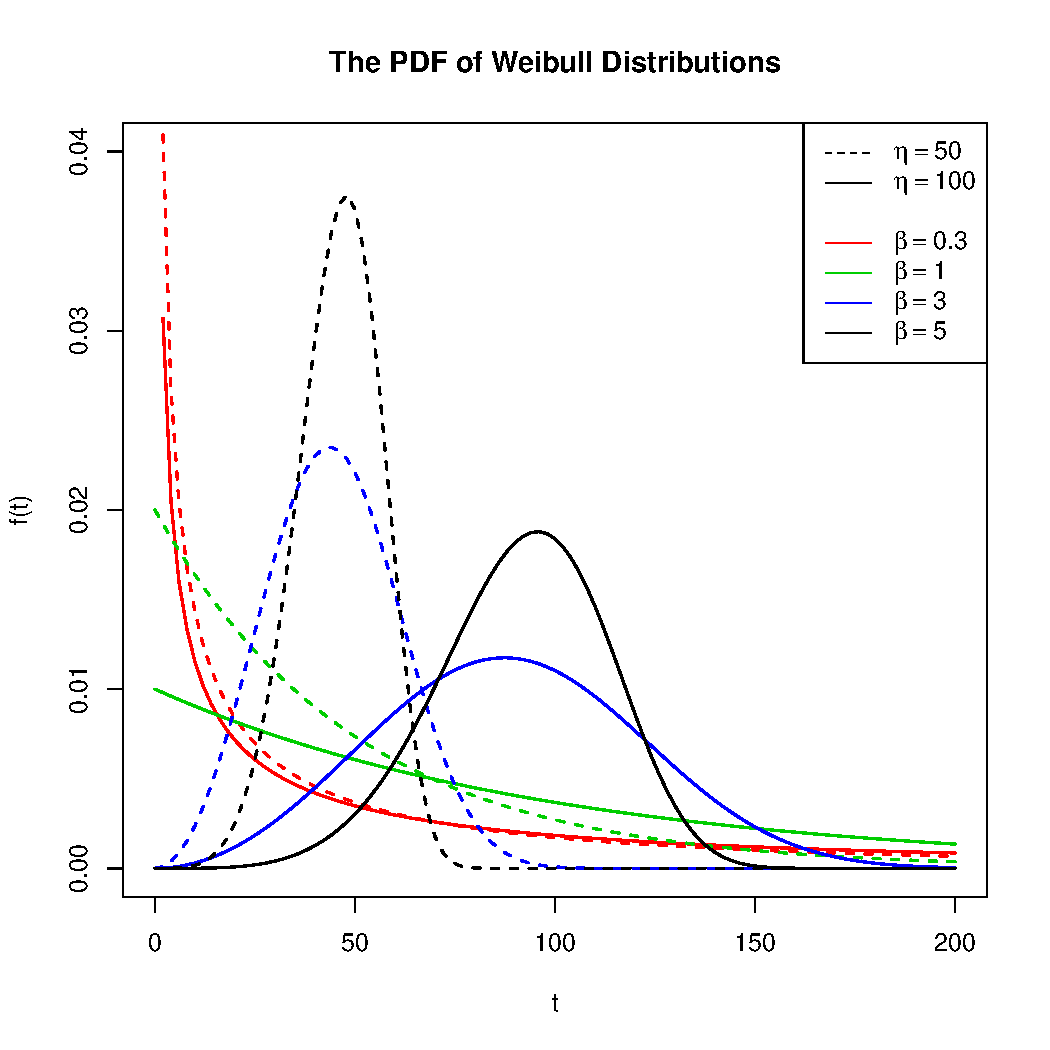
\includegraphics[width = \textwidth]{f_4_15_b.pdf}
\item[(c)]	For the fixed $\eta$, $F(t)$ converges to $0$ and $\gamma_2$ increases as $\beta$ increases.
\end{itemize}

%----------------------------------------------------------------------------------------
%	5.1
%----------------------------------------------------------------------------------------
5.1
\begin{itemize}
	\item[(a)]	\begin{align*}
				F(t; \bm{\theta}) &= \frac{1}{2}F(t; \theta_1) + \frac{1}{2}F(t; \theta_1)\\
							 &= \frac{1}{2}\left(1-exp(-t)\right) + \frac{1}{2}\left(1-exp\left(-\frac{t}{5}\right)\right)\\
							 &= 1- \frac{1}{2}\left( exp(-t) + exp\left(-\frac{t}{5}\right)\right)
			\end{align*}
	
	\item[(b)]	$$f(t; \bm\theta) = \frac{d}{dt} F(t; \bm\theta) =  \frac{1}{2}\left( exp(-t) + \frac{1}{5}exp\left(-\frac{t}{5}\right)\right)$$
	
	\item[(c)]	$$h(t; \bm\theta) = \frac{f(t; \bm\theta)}{1-F(t; \bm\theta)} = \frac{exp(-t) + \frac{1}{5}exp\left(-\frac{t}{5}\right)}{exp(-t) + exp\left(-\frac{t}{5}\right)}$$
	
	\item[(d)]	\ \\ 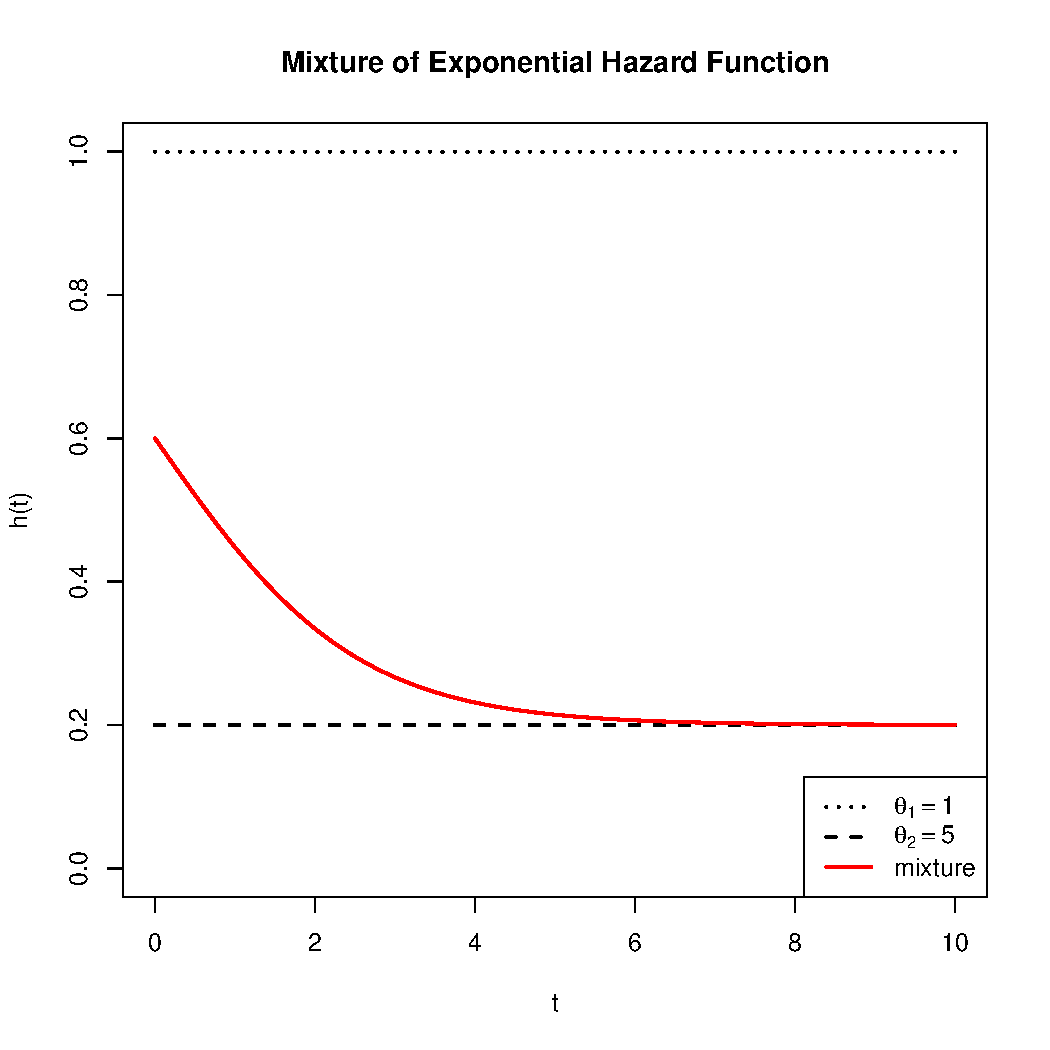
\includegraphics[width = \textwidth]{f_5_1_d.pdf}
	
	\item[(e)]	It is a strictly decreasing convex curve ranges from $0.2$ to $1$. 
	
	\item[(f)]	Its hazard is strictly decreasing and converges to $0.2$.
\end{itemize}

\newpage
%----------------------------------------------------------------------------------------
%	5.8
%----------------------------------------------------------------------------------------
5.8
\begin{itemize}
	\item[(a)]	$$X \sim Gamma(\alpha,\beta) \text{\ and\ } Y \sim Exp(X)$$
			\begin{align*} f_Y(y) &= \int_{x=0}^\infty f_{Y \mid X}(y \mid x) f_X(x) \, dx \\ &= \int_{x=0}^\infty x e^{-x y} \frac{\beta^\alpha x^{\alpha-1} e^{-\beta x}}{\Gamma(\alpha)} \, dx \\ &= \frac{\beta^\alpha}{\Gamma(\alpha)} \int_{x=0}^\infty x^{\alpha} e^{-(y+\beta)x} \, dx \\ &= \frac{\beta^\alpha \Gamma(\alpha+1)}{\Gamma(\alpha)(y+\beta)^{\alpha+1}} \int_{x=0}^\infty \frac{(y+\beta)^{\alpha+1} x^{\alpha} e^{-(y+\beta)x}}{\Gamma(\alpha+1)} \, dx \\ &= \frac{\alpha\beta^\alpha}{(y + \beta)^{\alpha+1}}  \\ F(t) &= \int_0^t \frac{\alpha\beta^\alpha}{(y + \beta)^{\alpha+1}} dy\\ &= \left. \alpha\beta^\alpha \frac{1}{-\alpha}\left( y+\beta \right)^{-\alpha -1} \right|_0^t \\ &= 1-\beta^\alpha \left( t+\beta \right)^{-\alpha} \\ &= 1- \frac{1}{\left( 1+ \frac{t}{\beta}\right)^{\alpha}} = 1- \frac{1}{\left(1+\theta t \right)^\kappa} \text{\ , where\ } \theta = \frac{1}{\beta} \text{\ and \ } \kappa = \alpha\end{align*}
			
	\item[(b)]	$$f(t; \theta, \kappa) = \frac{d}{dt} F(t; \theta, \kappa) = \kappa \theta \left( 1+\theta t \right)^{-\kappa-1} \text{, where } t>0.$$
	
	\item[(c)]	$$h(t; \theta, \kappa) = \frac{f(t; \theta, \kappa)}{1-F(t; \theta, \kappa)} = \frac{\kappa\theta}{1+\theta t}\text{, where } t>0.$$
\end{itemize}

%----------------------------------------------------------------------------------------
%	5.12
%----------------------------------------------------------------------------------------
5.12
\begin{itemize}
	\item[(a)]	Let $T_1$, $T_2$, ..., $T_m \sim Weilbull(\mu_i, \sigma)$, $i = 1, 2, ..., m$. 
			$$Y=min(T_1, T_2, ..., T_m)=T_{(i)}$$
			$$F(t) = 1-exp\left[-\left( \frac{t}{\mu_i}\right)^\sigma \right]$$
			$$S(t) = 1-F(t) = exp\left[-\left( \frac{t}{\mu_i}\right)^\sigma \right]$$
			
			\begin{align*}
				S_Y(y)	&=	P(Y \geq y) = P(T_{(1)} \geq y) \\
						&=	P(T_{(1)} \geq y, T_{(2)} \geq y, ..., T_{(m)} \geq y) \\
						&=	P(T_{(1)} \geq y)P(T_{(2)} \geq y), ..., P(T_{(m)} \geq y) \\
						&=	exp\left[-\left( \frac{t}{\mu_1}\right)^\sigma \right] \cdot
							exp\left[-\left( \frac{t}{\mu_2}\right)^\sigma \right] \cdots
							exp\left[-\left( \frac{t}{\mu_m}\right)^\sigma \right] \\
						&=	exp\left[-\sum_{i=1}^m\left( \frac{t}{\mu_i}\right)^\sigma \right]
			\end{align*}
			$$ F(y) = 1- S(y) = 1-exp\left[-\sum_{i=1}^m\left( \frac{t}{\mu_i}\right)^\sigma \right]$$
			Hence, $T_{(1)}$ has a Weilbull distribution with shape parameter $\sigma$ and scale parameter $\sum_{i = 1}^m\frac{1}{\mu_i}$.
\end{itemize}

%----------------------------------------------------------------------------------------
%	6.1
%----------------------------------------------------------------------------------------
6.1
\begin{itemize}
	\item[(a)]	Quantile: 	$$t_p = exp\left[ \mu + \sigma \Phi_{logis}^{-1}(p) \right]$$
					$$log(t_p) =  \mu + \sigma \Phi_{logis}^{-1}(p)$$
			The plot of $log(t_p)$ versus $\Phi_{logis}^{-1}(p)$ is a straight line.
	
	\newpage
	
	\item[(b)]	\ \\
			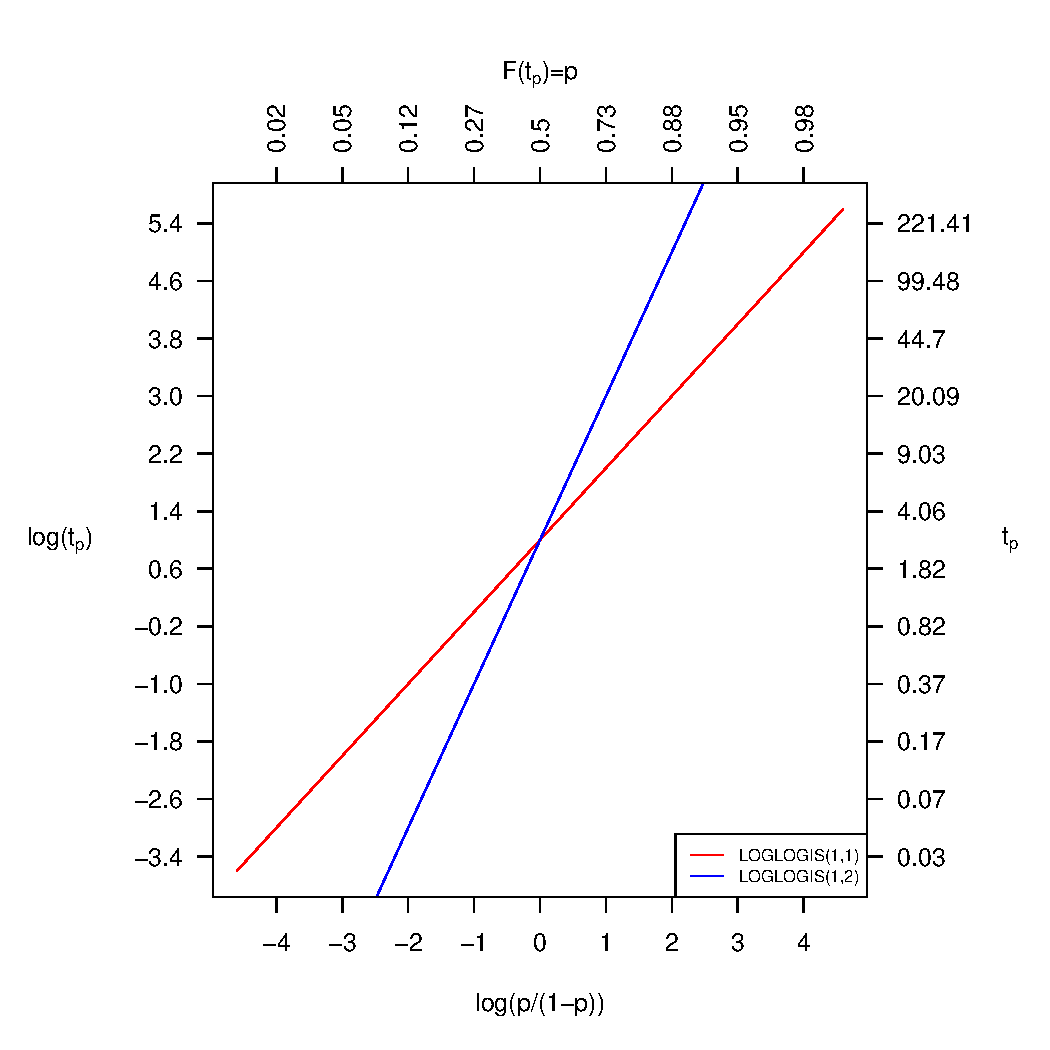
\includegraphics[width = \textwidth]{f_6_1_b.pdf}
			
	\item[(c)]	$$t_p = exp\left[ \mu + \sigma \Phi_{logis}^{-1}(p) \right]$$
\end{itemize}
%------------------------------------------------
\end{document}